\documentclass{article}
\usepackage{graphicx} % Required for inserting images
\usepackage{xcolor}
\usepackage{hyperref}
\usepackage{incgraph,tikz}
\usepackage{listings}
\usepackage{multicol}
\usepackage{biblatex} % Bibliography package
\addbibresource{bibliography.bib} % Bibliography file



\title{DevOps - Final Report\\
  \large Group I
}

\author{
Anders Latif (alat@itu.dk)\\
Ivar Cmrečak (ivcm@itu.dk)\\
Mads Meinert Andersen (mmea@itu.dk) \\
Mikkel Rahlff Berggreen (mirb@itu.dk)\\ 
Nedas Surkus (nesu@itu.dk)\\
}
\date{May 2023}


\begin{document}

\maketitle

\vspace*{\fill}
\noindent Course Name: DevOps, Software Evolution and Software Maintenance, MSc\\
Course Code: KSDSESM1KU\\
Github: \url{https://github.com/MinitwitGroupI/MiniTwit/}\\
Domain: \url{https://opsdev.gg}


\pagebreak

\tableofcontents
\pagebreak

\section{Problem formulation}

We have inherited a legacy system called Minitwit and have been tasked with refactoring it. Besides modernizing the stack it has been our aim to do so using DevOps methodologies. By reflecting on select few pillars of DevOps the final question becomes whether or not we achieved this goal; is what we've done DevOps?

\section{System's Perspective} 

\subsection{Design and architecture of the system}

Minitwit uses a container-based architecture where each service runs in its own Docker container. The web application is built with FastAPI and Jinja. Grafana and Prometheus are utilized for monitoring, the EFK stack for logging, Redis and PostgreSQL serve as database.

A deployment view was created to help illustrate how these components are deployed and interact with each other in a production environment.

\begin{figure}[h]
    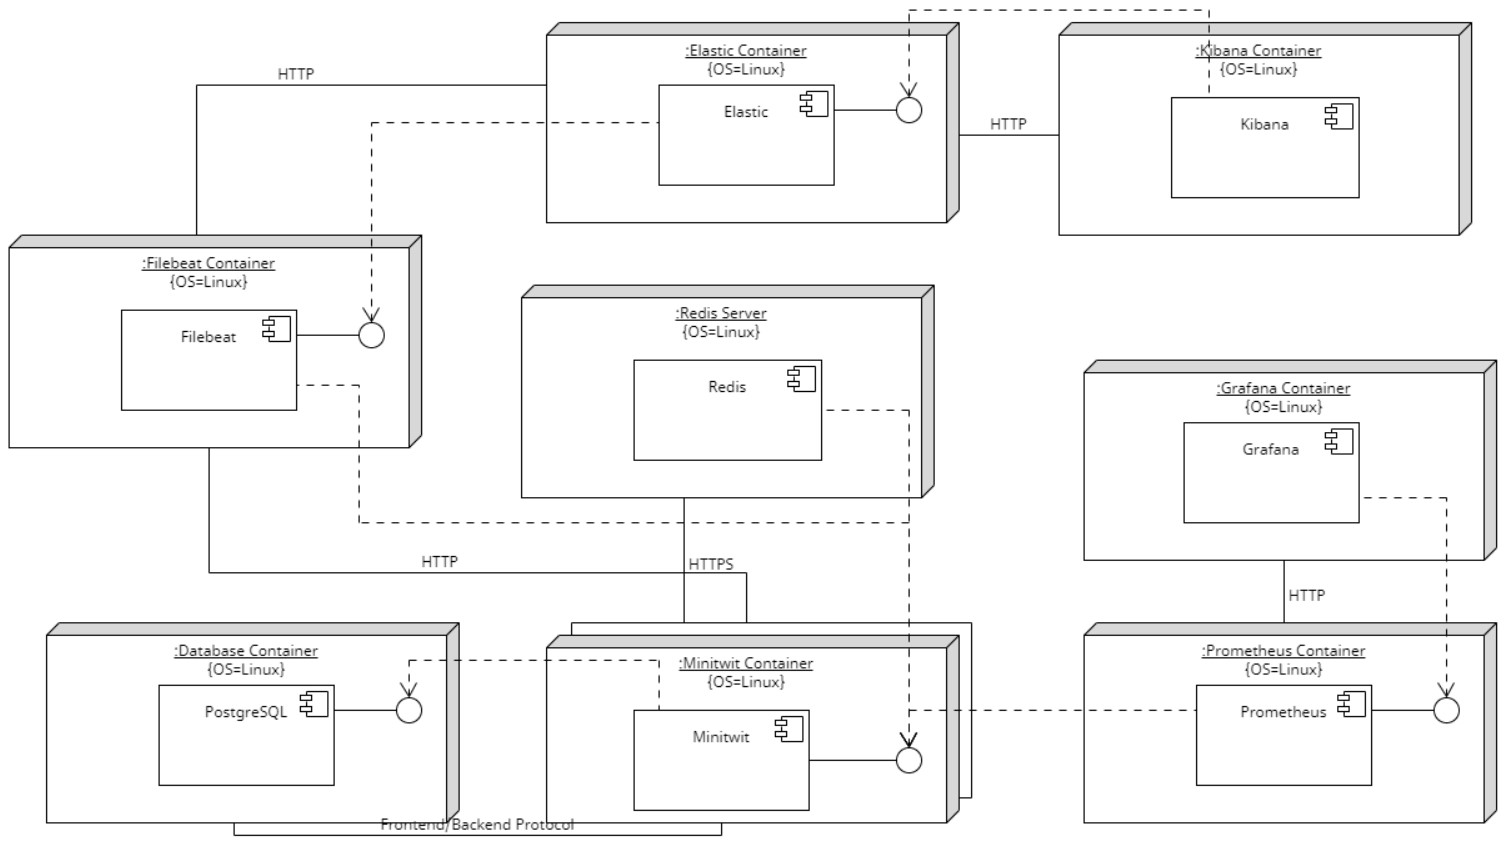
\includegraphics[width=1\textwidth]{images/DeploymentView2.0.jpg}
    \label{fig:ci_pipeline}
    \centering
    \caption{Component Diagram}
\end{figure}


\subsection{Dependencies of the system}

Technologies and tools:

\begin{multicols}{2}
\begin{itemize}
    \item FastAPI for the backend.
    \item PostgreSQL as database system.
    \item SQLAlchemy as an ORM framework.
    \item Docker for containerization.
    \item Vagrant for managing creation of virtual environments.
    \item DigitalOcean for hosting virtual environments on a remote server.
    \item GitHub Actions and Ansible for the CI/CD chain.
\end{itemize}
\vfill\null
\columnbreak
\begin{itemize}

    \item Prometheus and Grafana for monitoring and visualising the state of the system.
    \item Postman for testing API endpoints.
    \item Elasticsearch, Filebeat and Kibana as a logging stack.
    \item Redis for storing global state.
    \item Nginx and Heartbeat for a high-availablity setup with a staging and deployment server.
    \item Certbot for adding HTTPS to the website.
\end{itemize}
\vfill\null
\end{multicols}
Languages:
\begin{itemize}
    \item Python for the web application.
    \item Jinja as a templating language.
    \item Text for creating the Dockerfile.
    \item YAML for Docker, Ansible and Github Actions
\end{itemize}

\subsection{State of the system}

The application is accessible on \url{https://opsdev.gg}. The code can be found in \href{https://github.com/MinitwitGroupI/MiniTwit}{this repository}. Everything is running without error and will be accessible until the date June 14th 2023.
Our system has been able to process at least 12.778.829 \footnote{\url{http://opsdev.gg:3000/d/DVJQxp-4k/minitwit-responses?orgId=1&viewPanel=2}} events in the span of 8 weeks.

\subsection{Licences}

Since profiting is not our purpose the code is under the \href{https://github.com/MinitwitGroupI/MiniTwit/blob/main/LICENSE}{MIT License}.

\subsection{Weekly tasks}\label{WeeklyTasksSection}


\subsubsection{Week 1 - Bug fixing the old program}

By importing the project to IntelliJ it auto-suggested to update the Python version from 2 to 3 and automatically converted all code. We used shellcheck to lint the bash script. We fixed bugs related to tests not passing.

\subsubsection{Week 2 - Refactoring the app in another language }

We did two rounds of voting. Initially we listed all possible frameworks we wished to work with and then voted on which frameworks should be eliminated until we had 2 finalists and then used a roulette to pick between the two. The process is described here \footnote{\url{https://docs.google.com/document/d/1EOrFKD0XFW5gxv1NycgtTuj9rO6dggau99LybLYIRq0/edit\#heading=h.r8lyr8ciz36h }}. 

Fast API was chosen due to general familiarity with the framework, allowing the team to reuse Jinja and low amount of change needed to port the application to the framework. We could even reuse the Jinja templates. This would let us focus on the DevOps tasks rather than web development. 

We experienced some unexpected downsides to FastAPI:
\begin{itemize}
    \item The implementation of redirection for redirecting from a POST to another POST request would mean the loss of the original body and no way to pass it along. 
    \item Redirecting between different routes would return different status codes which created an unexpected challenge.
    \item Since it is multi-threaded server it excludes the ability to have a global state and a session. We solved it with Starlette Session but still caused limitations in regards to combining it with middleware.
    \item The tests required to be translated to Starlette framework in order to be utilised.
\end{itemize}

\subsubsection{Week 3 - Virtualisation and deployment to the server}

We created a single Dockerfile and set up Docker Compose. The old application was written for the Ubuntu 12.04 operating system, so for our deployment target we chose a DigitalOcean virtual machine using Ubuntu 22.04. DigitalOcean was chosen for it's ease of configuration and free student credits.

Initially, a new Docker feature called "Dev Environments" was used but it was  scraped as the environment prevented files mounting to containers and hot reloading.


\subsubsection{Week 4 - Setting up CI/CD system }

Github Actions gave us a simple configuration process without needing additional hosted infrastructure. Ansible was chosen for deploying our changes because of it's idempotency, declarative paradigm and simple configuration.
See section \ref{cicd}. 

Fetching secrets between Github Actions and Ansible were initially solved by creating a file on the server instead of storing all of them in Github Actions Secrets. This was only fixed in week 6.

\subsubsection{Week 5 - ORM }

Three ORMs have been considered and the arguments are mapped \footnote{\url{https://docs.google.com/document/d/1EOrFKD0XFW5gxv1NycgtTuj9rO6dggau99LybLYIRq0/edit\#heading=h.auxry4rgtrx1}}. A benchmark repository was created \footnote{\url{https://github.com/MinitwitGroupI/ORM_Benchmarks }} and after a Github Discussion \footnote{\url{https://github.com/MinitwitGroupI/MiniTwit/discussions/57 }} a vote was held. The choice fell on the most popular choice for Python - SQLAlchemy - which did not cause any notable issues. 

\subsubsection{Week 6 - Monitoring }

Prometheus with Grafana is considered the most popular choice in the industry \footnote{https://stackshare.io/stackups/grafana-vs-nagios}. 


FastAPI is both multi-threaded and stateless which excludes the ability to have a global state. Storing the total http calls would only pertain to the current thread. This was solved by storing the value in Redis. This was done in an asynchronous way that wouldn't impact performance. 

We audited our partner groups website and created issues for issues that were discovered \footnote{\url{https://github.com/organizationGB/DevOps/issues/23}} \footnote{\url{https://github.com/organizationGB/DevOps/issues/25}}. 

\subsubsection{Week 7 - Maintainability, external code analysing }

The Flake8 linter used by pylint does static code analysis in our CI pipeline to provide soft feedback that does that only blocks builds if there is any problems that would cause a crash, otherwise it provides hints on ways to improve current coding style. SonarQube and CodeClimate integrated perfectly with our repository but gave vastly different views on code quality than anticipated. It required manually dismissing a lot of warnings about duplicated code which existed in our unit tests and provided several false positives that had to be dismissed. It ended up being a burden rather than helpful.

\subsubsection{Week 8 - EFK stack}

The provided guide \footnote{https://github.com/itu-devops/itu-minitwit-logging} inspired us to go with the EFK stack. Significant issues were encountered during setup:

\begin{itemize}
    \item Adjustment of versions were required from the provided guide 
    \item Poor support for encoding custom user credentials in Kibana and Elastic Search.
    \item User credentials on Filebeat had to be manually hard coded.
    \item There was little documentation on what security features have to enabled in Production
    \item Any change could only be tested in production given our setup.
\end{itemize}

This meant that implementing the EFK stack was the most difficult and time consuming assignment. 

Implementing the EFK stack required vertically scaling the server in terms of CPU, memory and disk size. This resulted in server downtime of 1 day. 

The postmortem exercise was completed. A crash was introduced inside the "message" field and the logging was used to locate the crash point and patch it. \footnote{\url{https://github.com/MinitwitGroupI/MiniTwit/blob/main/docs/Postmortems.md}}. 

\subsubsection{Week 9 - Security assessment}

Metasploit and OWASP ZAP scans revealed minor vulnerabilities relating to missing headers for clickjacking.
\footnote{\url{https://github.com/MinitwitGroupI/MiniTwit/blob/main/docs/security\%20report/ZAP\%20Scanning\%20Report_1.pdf}}. 

The idea of integrating OWASP ZAP to the CI/CD pipeline was considered but dismissed on grounds of being beyond the scope.

A Lynis scan was carried out on the server which resulted in setting up Fail2ban. 

A security assessment was performed on our partner group. See Appendix section  \ref{appendix:securityAssessment}.\footnote{\url{https://github.com/MinitwitGroupI/MiniTwit/blob/main/docs/security\%20report/Group\%20I\%20\%20-\%20Security\%20Assessment\%20Findings\%20Report.pdf}}

\subsubsection{Week 10 - Scaling and rolling out updates }

We opted to go with the high-availability setup given the parameters of the project that included a fixed deadline and expectation of a reasonable amount of HTTP calls to handle. 

A scalable deployment would require refactoring several components of our stack. This would mean having a single server for the database which is costly but also creates a new single point of failure. 

We already implemented deployments to a staging environment prior to production, so adding the staging server to our high-availability setup also provided us with rolling updates. Rolling updates solved the ~1 min downtime experienced during every deployment.  

\subsubsection{Week 12 - Encode your infrastructure setup }

Changing our existing IaC from Vagrant to Terraform did not provide any perceived benefits. Vagrant works for both provisioning and configuration management. Besides the lack of benefits, the downside of Terraform is having to deal with state. 

\section{Process' perspective} \label{cicd}

\subsection{Team Organisation and Developer interaction} 

A Github organisation \href{https://github.com/MinitwitGroupI/}{MinitwitGroupI} was created and the team interaction was centered around Github and Discord. Discord was used for informal discussion and to make sure everyone is on the same page. For tasks and discussions Github Issues were encouraged. This gave us a Project View with a visual Kanban \footnote{\url{https://github.com/orgs/MinitwitGroupI/projects/1}}. 

\subsection{Stages and tools utilized in CI/CD chains}

We use GitHub Actions for performing all CI/CD operations.

\subsubsection{Continuous Integration (CI)}

Upon each commit, Github Actions triggers a job that builds our application using Docker. This process creates a Docker image, which is then used as the environment for linting and running unit tests on the Python code base. Integration tests are located in sim\_api\_test.py which creates a test database and tries the simulator endpoints.
UI tests can be located in minitwit\_old\_test.py which test out the functionality of all routes.



For a pull request to be merged, it must successfully pass all unit and integration tests.
\begin{figure}[h]
    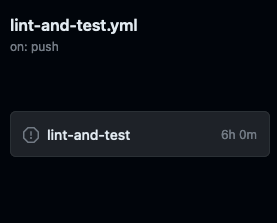
\includegraphics[width=0.4\textwidth]{images/Lint-and-test_Pipeline.png}
    \label{fig:ci_pipeline}
    \centering
    \caption{Lint and test pipeline}
\end{figure}
    

\subsubsection{Continuous Deployment (CD)}

An approved pull request to merge with the main branch triggers the CD pipeline. The first step in this pipeline is pushing the new versions of the Docker images to Docker Hub. 

Using Ansible, we first deploy our entire application stack to a staging server. This environment allows us to verify the functionality and stability of our application before deploying it to production.

After successful deployment to the staging server, we run liveness tests using Postman. These tests are designed to validate the overall health and performance of our application from a client perspective, ensuring that it meets the necessary requirements for production deployment. 

A passing liveness test is required to deploy to our production server. 

\begin{figure}[h]
    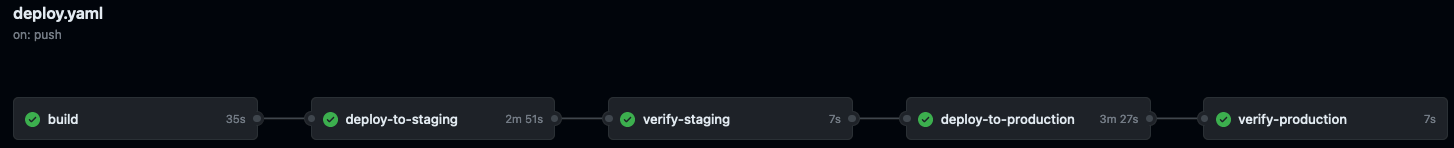
\includegraphics[width=1\textwidth, height=2.5cm]{images/Deploy_Pipeline.png}
    \label{fig:cd_pipeline}
    \caption{Deployment pipeline}
    \centering
\end{figure}

\subsection{Organization of the repository}

CONTRIBUTE.md explains the structure of the repository and our expectations for contributing to it \footnote{\url{https://github.com/MinitwitGroupI/MiniTwit/blob/main/docs/CONTRIBUTE.md}}. Everything is contained in a mono-repository.

\subsection{Branching strategy}

We use the feature branches strategy. For releases \footnote{https://github.com/MinitwitGroupI/MiniTwit/releases} we achieved trunk based development by pushing into main and manually bundling releases. In order to push to main, we had setup branch protection that require pull requests to be reviewed by at least one other team members, with the goal to attach anyone that would be involved with the task. Our branching philosophy is described here \footnote{https://github.com/MinitwitGroupI/MiniTwit/blob/main/docs/CONTRIBUTE.md}.

\subsection{Monitoring}

We use Grafana, Prometheus and Kibana to gather and visualize data.

The main dashboard can be found here\footnote{\url{http://opsdev.gg:3000/d/DVJQxp-4k/minitwit-responses?orgId=1&from=now-24h&to=now}}.

The metrics are inspired by the Google Site reliability engineering standard called 4 golden signals \footnote{\url{https://sre.google/sre-book/monitoring-distributed-systems/\#xref_monitoring_golden-signals}}.

\begin{enumerate}
    \item \textbf{Latency}: Response times and request duration distribution.
    \item \textbf{Traffic}: Endpoint hits and total number of requests.
    \item \textbf{Errors}: Monitoring error logs as a percentage total requests
    \item \textbf{Saturation}: CPU usage.
\end{enumerate}
Appendix \ref{appendix:monitoringDashboard} shows an overview. 
\newline

Postman runs daily on the production frontend and sends emails if anything is down. As part of the Postman monitoring we test response time and this helped us notice that our front page load times were extremely slow. This was solved by adding indexes in the database to the field "pub\_date desc" and "author\_id". 

\subsection{Logging}

For logging we use the EFK stack. The Kibana dashboard can be found on \url{http://opsdev.gg:5601} with the username \emph{helgeandmircea} and password \emph{sesame0uvr3toi}. 

We aggregate multiline logs into a single log in FileBeat and filter them inside Kibana using several regex filters. The dashboards were created using Kibana's dashboard visualization tool. Appendix \ref{appendix:loggingDashboard} shows an overview.


\subsection{Security Assessment}

From the view of DevSecOps, security is an integral part of the development life cycle. We created a risk analysis review. Furthermore, here are the result of security assessment: 

\begin{itemize}
    \item Scanning our application with Metasploit and OWASP ZAP highlighted some missing headers to prevent clickjacking, but no significant vulnerabilities. 
    \item The assigned peer team attempted to exploit the website but did not produce any noteworthy results. 
    \item Conducting a review on the teams assigned peer team resulted in the other teams database and cookies being compromised. We go into depth in the appendix \ref{appendix:securityAssessment}.
\end{itemize}


\subsection{Scaling and Load balancing}

We have opted out of a scalable setup since this would require us to heavily refactor our infrastructure and separate our database from individual nodes. This would cost more with no added benefit in the confinement of the expected user growth before the deadline.  

\subsection{High-availability setup}

We have opted for a high-available setup by using Heartbeat following a guide provided by DigitalOcean \footnote{https://www.digitalocean.com/community/tutorials/how-to-create-a-high-availability-setup-with-heartbeat-and-reserved-ips-on-ubuntu-16-04}. This utilizes `floatip` which uses the DigitalOcean API to update the reserved IP to point at the other server when one is unavailable. 

\begin{figure}[h]
    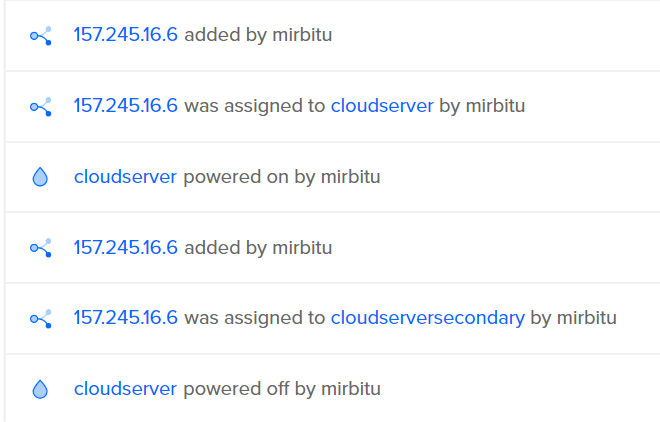
\includegraphics[scale=0.7]{images/Heartbeat_Working.png}
    \label{fig:cd_pipeline}
    \caption{Heartbeat reassigning the reserved IP}
    \centering
\end{figure}

\section{DevOps principles}\label{DevOpsPrinciplesSection}

\subsection{What is DevOps}

Going by the DevOps Handbook \cite{devopshandbook} we have chosen a couple defining concepts in flow, feedback and continual learning and experimentation to compare our result against. 

\subsection{Ways we are DevOps}

\subsubsection{Flow}

\begin{enumerate}
    \item Make work visible: We used the kanban provided by Github Project for feature development. 
    \item Limit Work in Progress: The course structure helped spread out the tasks. After each exercise session, team members would create new issues that need to be implemented or fixed.
\end{enumerate}

\subsubsection{Feedback}

See Problems as They Occur: 

\begin{enumerate}
    \item We set up monitoring and logging.
    \item The repository also features badges that display if the pipelines fail or succeed. Deployment to production is aborted in case of failure in the staging environment.
\end{enumerate}

\subsubsection{Collaborating}

Make use of software development approaches:

\begin{enumerate}
    \item Pair-Programming
    \item Mob Programming
\end{enumerate}

\subsubsection{Continual Learning and experimentation}

Considering the small team and constant change in weekly tasks this was not a corner stone of our DevOps approach. 

\subsection{Ways we are not DevOps}

We have not focused on anything relating to the Toyota Kata\footnote{ The DevOps Handbook. Page 6-8.} and seeing our development as a value stream that could contain waste. 

While Github Issues were created for features, ad hoc tasks such as hot fixes were not, which breaks the principle of making work visible. 

\subsubsection{Knowledge transfer}

"The Bus Factor" was repeated during the guest lecture which is the concept that no single developer should become key to development or infrastructure to the degree that progress can't occur without them. We did have insufficient knowledge transfer across the team but not to such a severe degree that it could be termed "The Bus Factor".

We each carved out our niche based on prior knowledge. PR reviews were intended for knowledge sharing but had its limitations. We tried to amend this by creating good documentation in our repository for each other, but some of the non-standard solutions meant that a larger effort was required for role shifting.  

\subsubsection{Pushing Quality Closer to the Source}

SonarQube and CodeClimate were added and integrated with our repository, but ultimately ignored, because the warnings given were mostly non-applicable to the application. Likewise, we had set up linting but it was ignored as it was implemented late in the development cycle. We should've created a pre-commit hook that didn't allow pushing before all linting passes. 

\subsubsection{Reduce Batch Sizes}

During the course we were recommended to push daily. It was agreed upon in our team that this was not a key principle that we should adhere to. This was caused by having other conflicting obligations and only being able to work in spurts. 

Some tasks were split up into multiple stages:

\begin{enumerate}
    \item The ORM was integrated over the weeks while slowly phasing out the raw SQL queries. This gave room for writing corresponding tests. 
    \item The monitoring was done in two steps (backend and dashboard). This could've been split into even smaller commits. 
    \item The EFK task was split into three major phases: configuration / backend, deployment and dashboards.
\end{enumerate}

\noindent But some features were built completely before being merged:

\begin{enumerate}
    \item CI was merged only when we had working pipelines for both linting and testing.
    \item CD was merged only when it was successfully deploying all components to production.
\end{enumerate}

In conclusion, we could've approached the larger tasks in smaller batches.

\subsubsection{Psychological Safety}

DevOps has enjoyed many different views through different eras \cite{devopsviewsthrougheras}. The Phoenix Project \cite{thephoenixproject} focuses on DevOps as a culture. One important concept should be psychological safety.

It took time for us to align expectations. During this period we had to agree on the technology stack which felt like a popularity contest for the best framework. In the following weeks however, everyone became really helpful and Discord calls occurred in random constellations. We picked up the term "psychological safety" from the guest lecture and repeated it as a mantra in our group.

\section{Lessons Learned Perspective}

\subsection{Issues and lessons learned}

\subsubsection{Refactoring} 

Picking FastAPI resulted in significantly less time spent on refactoring which allowed us to reuse big parts of the original Flask application. While Flask would've sufficed we managed to add better security through password encryption. 

\subsubsection{Evolution}

We were often blocked by upcoming tasks. Testing required implementing the ORM to mock a similar database setup as the one in production. We couldn't implement CI without tests and CD required CI to be done. 

In retrospect it's difficult to say if there is a better path to complete the project. It has become apparent to us which tasks were of the highest priority and that other tasks depended on. 

\subsubsection{Maintenance}

We have estimated the likely uptime based on Postman monitors and our monitoring dashboard and used the metrics in our SLA\footnote{https://github.com/MinitwitGroupI/MiniTwit/blob/main/docs/SLA.md}. 

Thanks to our monitoring we picked up on some infrequent outages. We could not verify whether some were caused by the simulator pausing or a problem on our end. We experienced at least three types of known outages:

\begin{enumerate}
    \item Outage during deployment while the Docker image was pulled and started. This was solved by our high-availability setup. 
    \item An initial misconfiguration of heartbeat caused CPU overprovisioning and huge latency issues.
    \item The daily 5 AM outage. Through research we discovered that PostgreSQL by default restarts and does garbage collection and other maintanance. 
\end{enumerate}

Overall we felt that a minimal amount of maintenance is needed and would confidently hand over the project to another team. 

\subsection{Reflection}

We reflect on our technology choices in \ref{WeeklyTasksSection}.
We reflect on how much we adhere to DevOps principles in \ref{DevOpsPrinciplesSection}.

In other university courses, there's not a big focus on team collaboration, so we entered the project without a baseline on how to work together.

We had hoped that PRs would ensure a high code quality, but with no prior experience with the technologies and obligations from other courses, we couldn't ensure a high standard was maintained. This let to the "lgtm" (looks good to me) syndrome.

Optimally we should have had a test environment as well as a production environment. Some changes would have unpredictable interactions only when deployed to production and as result would cause downtime.  Ensuring a test environment would have helped to mitigate this issue.

Before implementing CD we had a pull-based approach of the weekly release that would frequently break. Pinpointing the issue would mean having to go through all the commits which caused a long MTTR (mean time to repair). 

Due to budget constraints, we had to keep our persistent state on the same server as our stateless services. Decoupling the database from the rest of the infrastructure would give the additional benefit of easier implementation of scaling. 

It would've been nice to automate the infrastructure. Right now deploying from scratch requires some manual configuration. We wish IaC was created prior to main development. 


\subsection{Hand over}

We consider that no further maintenance is required. If a new group were to inherit our codebase, we have created a document to guide them. See Appendix section \ref{appendix:handOverGuide}. 

\section{Conclusion}

We have listed many technologies and tools that are typical of DevOps project. In isolation they do not make our work "DevOps". Instead it is in the way they flow seamlessly to provide Continuous Delivery and Continuous Feedback as part of The DevOps Way. We have also reviewed our team work through the lense of DevOps as a culture. We have reflected on possible improvement in how we work as a team as well as split up our commits in smaller batch sizes. Overall, we can conclude that our approach to the project has adhered to the principles of DevOps. 


\pagebreak
\printbibliography


\pagebreak
\section{Appendix}
\appendix


\section{Deployment View}
See next page
\label{appendix:DeploymentView}
\incgraph[documentpaper]
  [width=\paperwidth,height=\paperheight]{images/DeploymentView2.0.jpg}


\section{Hand over guide}
\label{appendix:handOverGuide}
Parts that need to be set up to inherit the codebase and deploy to a cloud server:
\begin{itemize}
    \item Local envionment variables: SSH\_KEY\_NAME, DIGITAL\_OCEAN\_TOKEN and AUTH\_KEY\_HEARTBEAT.
    \item GitHub Action Secrets: SSH\_HOST and STAGING\_SSH\_HOST.
\end{itemize}
To then deploy to a cloud server (in DigitalOcean), the "cloud\_deployment.md" guide in the GitHub repository should be followed.

In case the whole project is taken over, the following GitHub Actions Secrets would need to be set up:
\begin{itemize}
    \item DOCKER\_PASSWORD
    \item DOCKER\_USERNAME
    \item ELASTICSEARCH\_PASSWORD
    \item ENCRYPTION\_KEY
    \item PAT
    \item POSTGRES\_DB
    \item POSTGRES\_PASSWORD
    \item POSTGRES\_PORT
    \item POSTGRES\_SERVER
    \item POSTGRES\_USER
    \item POSTMAN\_API\_KEY
    \item REDIS\_HOST
    \item REDIS\_PASSWORD
    \item REDIS\_PORT
    \item SESSION\_SECRET\_KEY
    \item SSH\_HOST
    \item SSH\_KEY
    \item SSH\_USER
    \item STAGING\_SSH\_HOST
\end{itemize}

\section{Security Assessment (Partner Group)}
\label{appendix:securityAssessment}

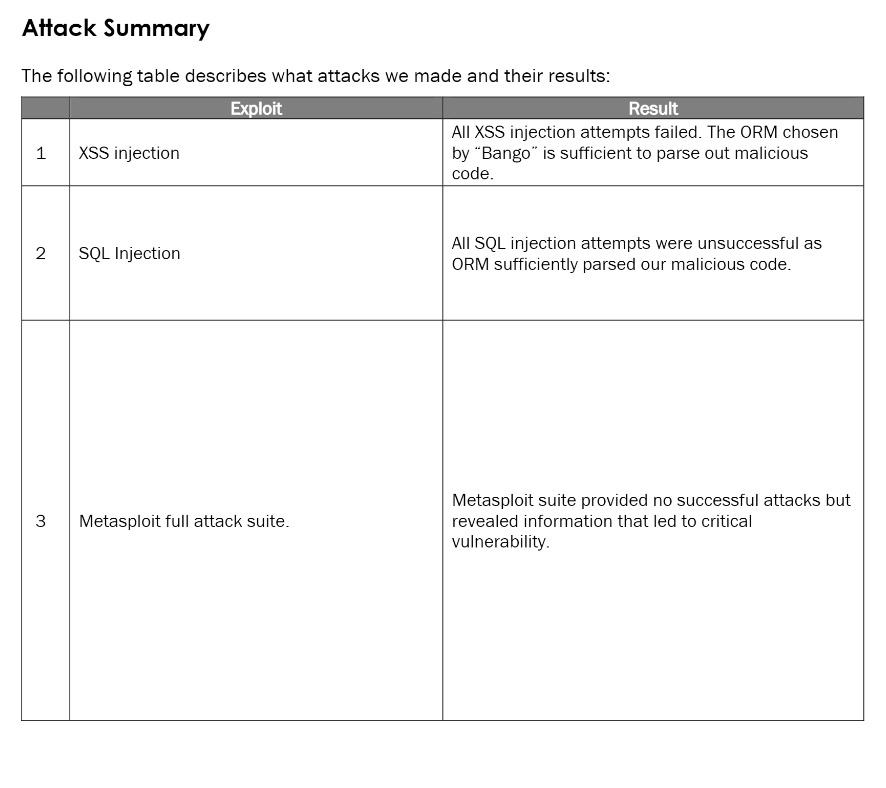
\includegraphics[width=1\textwidth]{images/Attack P1.png}

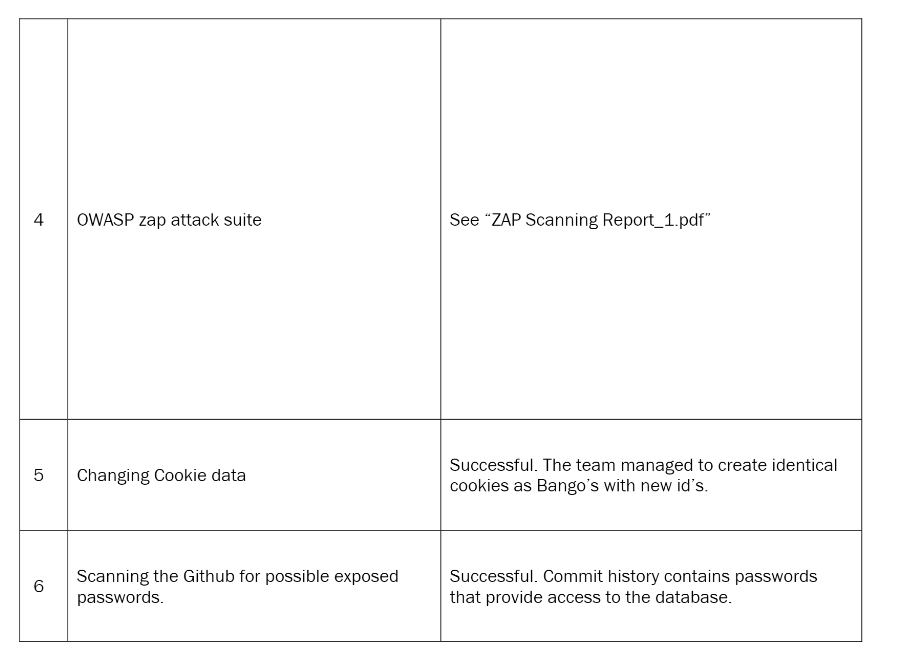
\includegraphics[width=1\textwidth]{images/Attack P2.png}
Read more :  \url{https://github.com/MinitwitGroupI/MiniTwit/blob/main/docs/security\%20report/Group\%20I\%20\%20-\%20Security\%20Assessment\%20Findings\%20Report.pdf}
\section{Current state of the application}
\label{appendix:currentState}
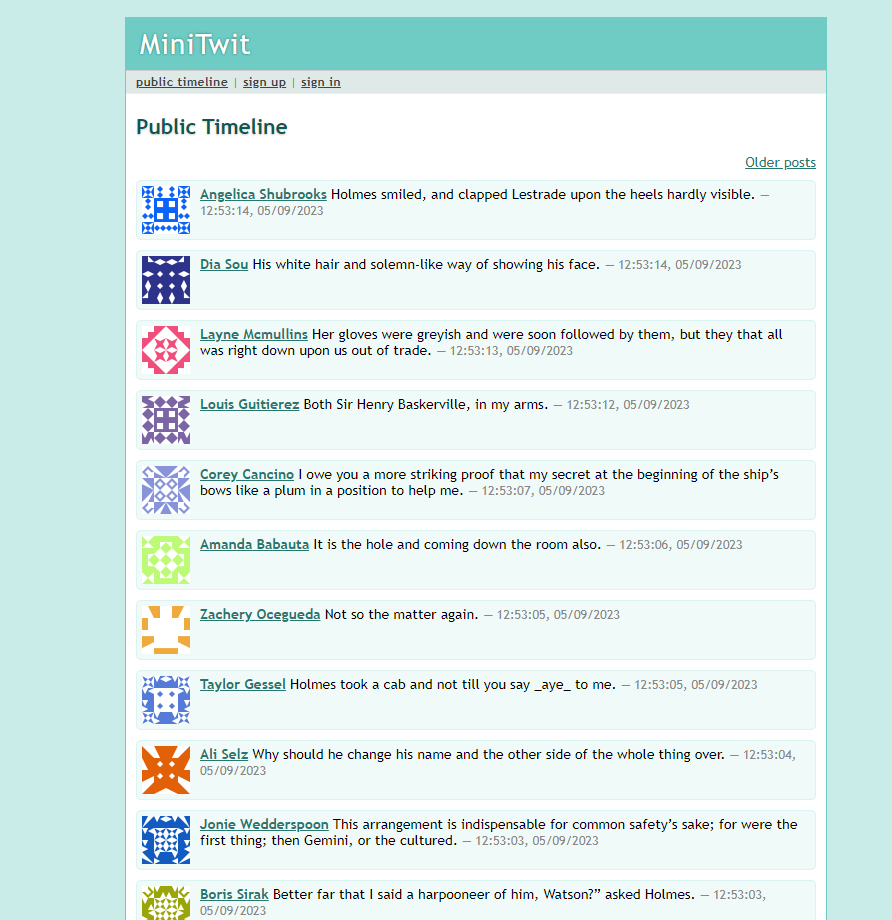
\includegraphics[width=1\textwidth]{images/OpsDev_screenshot.png}

\section{Monitoring Dashboard}
\label{appendix:monitoringDashboard}
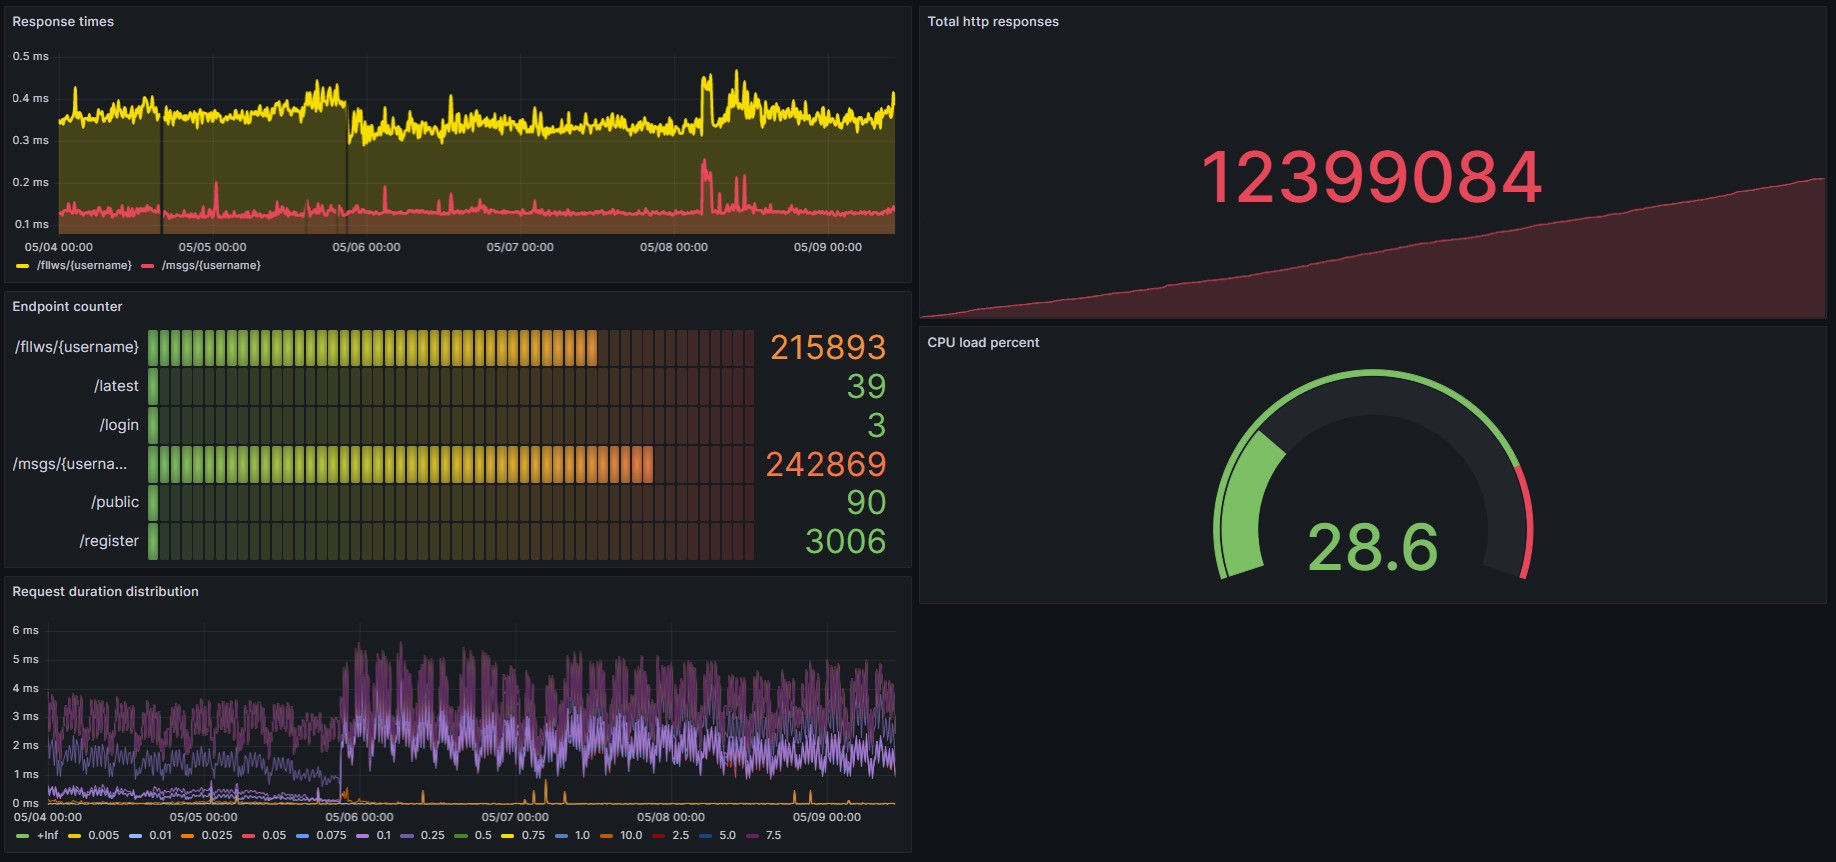
\includegraphics[width=1\textwidth]{images/MonitoringDashboard.jpg}

\section{Logging Dashboard}
\label{appendix:loggingDashboard}
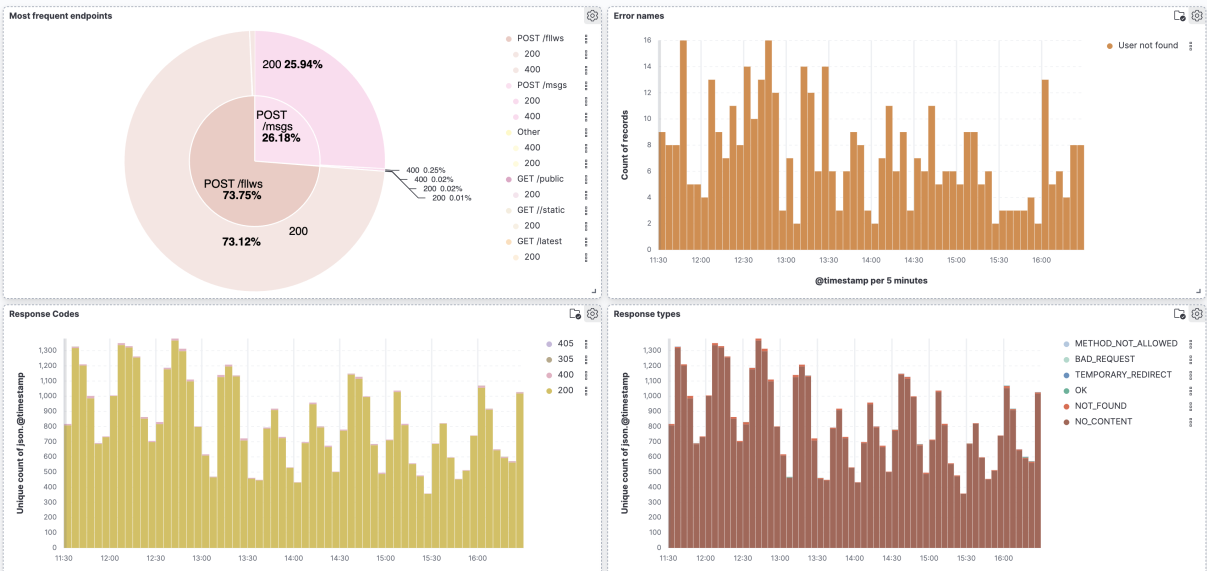
\includegraphics[width=1\textwidth]{images/LoggingDashboard.png}





\end{document}



